\chapter{Struktura zásuvného modulu}
\label{struktura_pluginu}

%% TODO - vymazat adresare, ktere nebudou v pluginu

\begin{minipage}{0.9\textwidth}
  \dirtree{%
  .1 /.
  .2 data/.
  .3 bpej/.
  .4 \detokenize{SC_BPEJ.csv}.
  .3 icons/.
  .4 checkanalysis.png.
  .4 edit.png.
  .4 loadvfk.png.
  .3 qml/.
  .4 PAR.qml.
  .4 perimeter.qml.
  .3 sql/.
  .4 \detokenize{add_pu_columns_PAR.sql}.
  .4 \detokenize{check_gc_srs.sql}.
  .4 \detokenize{check_pu_columns_PAR.sql}.
  .4 \detokenize{create_fill_gc_srs.sql}.
  .4 \detokenize{create_sobr_spol.sql}.
  .2 docs/.
  .2 .git/.
  .2 pubin/.
  .2 text/.
  .2 zadani/.
  .2 .gitignore.
  .2 \detokenize{__init__.py}.
  .2 metadata.txt.
  .2 puplugin.cfg.
  .2 puplugin.png.
  .2 puplugin.py.
  .2 puplugin.svg.
  .2 README.md.
  }
\end{minipage}

\begin{description}
	\item[\texttt{data}:] Složka obsahující všechna data.
	\begin{description}[leftmargin=1cm]
		\item[\texttt{bpej}:] Složka obsahující data pro~analýzu \textit{oceňování podle BPEJ}.
		\begin{description}[leftmargin=1cm]
			\item[\texttt{\detokenize{SC_BPEJ.csv}}:] Číselník \zk{BPEJ}.
		\end{description}
		\item[\texttt{icons}:] Složka obsahující ikony záložek.
		\begin{description}[leftmargin=1cm]
			\item[\texttt{checkanalysis.png}:] Ikona záložky \textit{Kontroly a analýzy}.
			\item[\texttt{edit.png}:] Ikona záložky \textit{Editace}.
			\item[\texttt{loadvfk.png}:] Ikona záložky \textit{Načtení VFK souboru}.
		\end{description}
		\item[\texttt{qml}:] Složka obsahující QML soubory.
		\begin{description}[leftmargin=1cm]
			\item[\texttt{PAR.qml}:] QML soubor pro~vrstvu \texttt{\zk{PAR}}.
			\item[\texttt{perimeter.qml}:] QML soubor pro~vrstvu obvodu.
		\end{description}
		\item[\texttt{sql}:] Složka obsahující SQL dávky.
		\begin{description}[leftmargin=1cm]
			\item[\texttt{\detokenize{add_pu_columns_PAR.sql}}:] SQL dávka pro přidání vlastních sloupců.
			\item[\texttt{\detokenize{check_gc_srs.sql}}:] SQL dávka pro kontrolu přítomnosti tabulek \textit{\detokenize{geometry_columns}} a~\textit{\detokenize{spatial_ref_sys}}.
			\item[\texttt{\detokenize{check_pu_columns_PAR.sql}}:] SQL dávka pro~kontrolu přítomnosti vlastních sloupců.
			\item[\texttt{\detokenize{create_fill_gc_srs.sql}}:] SQL dávka pro~vytvoření a~naplnění tabulek \textit{\detokenize{geometry_columns}} a~\textit{\detokenize{spatial_ref_sys}}.
			\item[\texttt{\detokenize{create_sobr_spol.sql}}:] SQL dávka pro~vytvoření tabulek \zk{SOBR} a~\zk{SPOL}.
		\end{description}
	\end{description}
	\item[\texttt{docs}:] Složka obsahující návod k~zásuvnému modulu.
	\item[\texttt{.git}:] Složka verzovacího systému Git.
	\item[\texttt{pubin}:] Složka vytvořeného Python balíčku, více viz příloha \ref{popis_python_balicku}.
	\item[\texttt{text}:] Složka obsahující text práce.
	\item[\texttt{zadani}:] Složka obsahující zadání práce.
	\item[\texttt{.gitignore}:] Soubor verzovacího systému Git pro~ignorování souborů.
	\item[\texttt{\detokenize{__init__.py}}:] Modul pro~inicializaci zásuvného modulu.
	\item[\texttt{metadata.txt}:] Soubor obsahující metadata o~zásuvném modulu.
	\item[\texttt{puplugin.cfg}:] Konfigurační soubor zásuvného modulu.
	\item[\texttt{puplugin.png}:] Ikona zásuvného modulu ve~formátu PNG.
	\item[\texttt{puplugin.py}:] Hlavní Python modul zásuvného modulu.
	\item[\texttt{README.md}:] Soubor obsahující základní informace o~repozitáři.
\end{description}

\chapter{Popis vytvořeného Python balíčku}
\label{popis_python_balicku}

Všechny třídy a~metody balíčku mají svůj vlastní \textit{docstring}, tedy komentář, ve~kterém je stručne napsáno, k~čemu třída či~metoda slouží, jaké má vstupní hodnoty, jaké vyvolává výjimky a~co za~hodnoty vrací. Při~vytváření těchto komentářu bylo vycházeno z~\textit{Google Python Style Guide}\footnote{\url{https://google.github.io/styleguide/pyguide.html}}.

Plugin se bude dále vyvíjet, proto jsou zde popsány pouze základní informace, díky kterým je možné se v balíčku a modulech orientovat.

\bigskip

\begin{minipage}{0.9\textwidth}
  \dirtree{%
  .1 pubin/.
  .2 pustack/.
  .3 puca/.
  .4 \detokenize{__init__.py}.
  .4 \detokenize{area_pucawidget.py}.
  .4 \detokenize{bpej_pucawidget.py}.
  .4 \detokenize{distance_pucawidget.py}.
  .4 \detokenize{notinmap_pucawidget.py}.
  .4 \detokenize{notinspi_pucawidget.py}.
  .4 \detokenize{perimeter_pucawidget.py}.
  .4 pucawidget.py.
  .4 \detokenize{unowned_pucawidget.py}.
  .3 \detokenize{__init__.py}.
  .3 \detokenize{checkanalysis_puwidget.py}.
  .3 \detokenize{edit_puwidget.py}.
  .3 \detokenize{execute_thread.py}.
  .3 \detokenize{load_thread.py}.
  .3 \detokenize{loadvfk_puwidget.py}.
  .3 puwidget.py.
  .2 \detokenize{__init__.py}.
  .2 dockwidget.py.	
  .2 stackedwidget.py.
  .2 statusbar.py.
  .2 toolbar.py.
  }
\end{minipage}

\begin{description}
	\item[\texttt{pubin}:] Hlavní Python balíček, který obsahuje všechny vytvořené moduly.
	\begin{description}[leftmargin=1cm]
		\item[\texttt{pustack}:] Balíček obsahující moduly všech záložek a~jimi používaných tříd. Třídy záložek dědí z~abstraktní bázové třídy \texttt{PuWidget} nacházející se v~modulu \texttt{puwidget.py}.
		\begin{description}[leftmargin=1cm]
			\item[\texttt{puca}:] Balíček obsahující moduly záložky \textit{Kontroly a~analýzy}. Písmena \texttt{ca} jsou zkratkou pro~anglický název záložky - \texttt{CheckAnalysis}. Všechny třídy kontrol a~analýz dědí z abstraktní bázové třídy \texttt{PuCaWidget} nacházející se v~modulu \texttt{pucawidget.py}. Pro spuštění kontroly nebo~analýzy slouží metoda \texttt{execute}.
			\begin{description}[leftmargin=1cm]
				\item[\texttt{\detokenize{__init__.py}}:] Modul pro~inicializaci balíčku.
				\item[\texttt{\detokenize{area_pucawidget.py}}:] Modul pro~kontrolu \textit{výměra nad~mezní odchylkou}.
				\item[\texttt{\detokenize{bpej_pucawidget.py}}:] Modul pro~analýzu \textit{oceňování podle BPEJ}.
				\item[\texttt{\detokenize{distance_pucawidget.py}}:] Modul pro~analýzu \textit{měření vzdálenosti}.
				\item[\texttt{\detokenize{notinmap_pucawidget.py}}:] Modul pro~kontrolu \textit{není v~mapě}.
				\item[\texttt{\detokenize{notinspi_pucawidget.py}}:] Modul pro~kontrolu \textit{není v~SPI}.
				\item[\texttt{\detokenize{perimeter_pucawidget.py}}:] Modul pro~kontrolu \textit{obvodem}.
				\item[\texttt{pucawidget.py}:] Abstraktní bázová třída, ze~které dědí všechny třídy kontrol a~analýz.
				\item[\texttt{\detokenize{unowned_pucawidget.py}}:] Modul pro~kontrolu \textit{bez~vlastníka}.
			\end{description}
			\item[\texttt{\detokenize{__init__.py}}:] Modul pro~inicializaci balíčku.
			\item[\texttt{\detokenize{checkanalysis_puwidget.py}}:] Modul pro~záložku \textit{Kontroly a~analýzy}.
			\item[\texttt{\detokenize{edit_puwidget.py}}:] Modul pro~záložku \textit{Editace}.
			\item[\texttt{\detokenize{execute_thread.py}}:] Modul pro~spouštění procesů editace, kontrol a~analýz v~samostatném vlákně.
			\item[\texttt{\detokenize{load_thread.py}}:] Modul pro~spouštění procesu načítání \zk{VFK} souboru v~samostatném vlákně.
			\item[\texttt{\detokenize{loadvfk_puwidget.py}}:] Modul pro~záložku \textit{Načtení VFK souboru}.
			\item[\texttt{puwidget.py}:] Abstraktní bázová třída, ze~které dědí všechny třídy záložek.
		\end{description}
		\item[\texttt{\detokenize{__init__.py}}:] Modul pro~inicializaci balíčku.
		\item[\texttt{dockwidget.py}:] Modul pro~hlavní grafickou komponentu pluginu.
		\item[\texttt{stackedwidget.py}:] Modul pro~grafickou komponentu, která obsahuje všechny záložky.
		\item[\texttt{statusbar.py}:] Modul pro~stavový řádek.
		\item[\texttt{toolbar.py}:] Modul pro~ikony na~přepínání mezi záložkami a~sadu standardních nástrojů programu QGIS.
	\end{description}
\end{description}

\chapter{Uživatelský manuál}
\label{uzivatelsky_manual}

\section{Instalace}
\label{manual_instalace}

Zásuvný modul není součástí oficiálního repozitáře QGIS, přesto ho lze nainstalovat stejným způsobem jako~jiné pluginy. Stačí do~programu QGIS přidat repozitář organizace GeoForAll Lab\footnote{\url{http://geomatics.fsv.cvut.cz/research/geoforall/}}.

Nejprve je tedy nutné otevřít okno s~repozitáři \textit{Zásuvné moduly $\rightarrow$ Spravovat a~instalovat zásuvné moduly $\rightarrow$ Nastavení} (viz obr.~\ref{fig:pridani_repozitare}) a~zde pomocí tlačítka \textit{Přidat...} doplnit repozitář GeoForAll Lab dostupný na~adrese:

\begin{lstlisting}[basicstyle=\footnotesize\ttfamily, backgroundcolor = \color{light-gray},  numbers=left]
http://geo.fsv.cvut.cz/geoforall/qgis-plugins.xml
\end{lstlisting}

Zásuvný modul se řadí mezi experimentální, proto je zapotřebí aktivovat volbu \textit{Zobrazit také experimentální zásuvné moduly}, viz obr.~\ref{fig:pridani_repozitare}. Poté už stačí do~vyhledávacího pole zadat \textit{PU Plugin} a~zásuvný modul pro~pozemkové úpravy nainstalovat (viz obr.~\ref{fig:instalace_puplugin}).

	\begin{figure}[H]
		\centering
		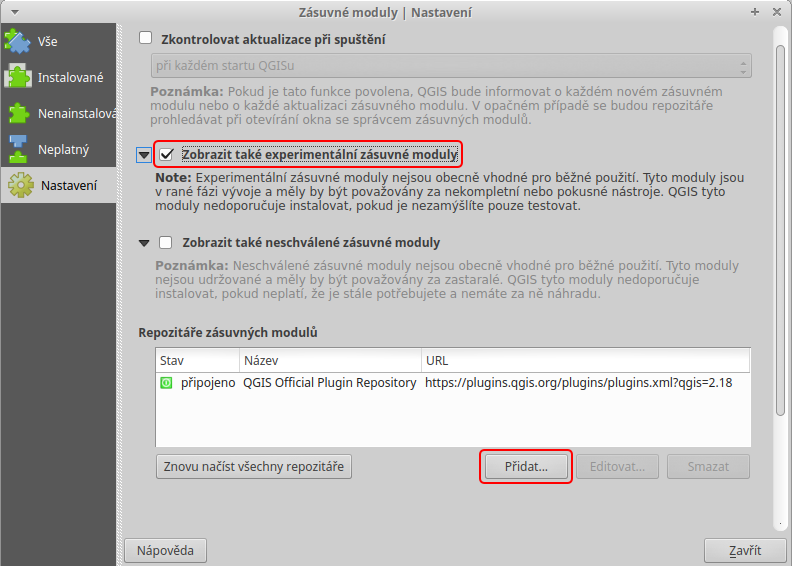
\includegraphics[width=.9\textwidth]{./pictures/pridani_repozitare.png}
		\caption[Přidání repozitáře]{Přidání repozitáře}
		\label{fig:pridani_repozitare}
 	\end{figure}
 	
	\begin{figure}[H]
		\centering
		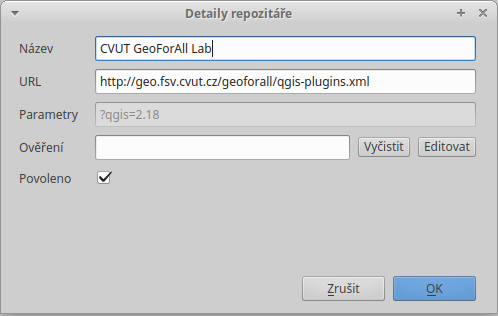
\includegraphics[width=.6\textwidth]{./pictures/pridani_repozitare-geoforall_lab.png}
		\caption[Přidání repozitáře GeoForAll Lab]{Přidání repozitáře GeoForAll Lab}
		\label{fig:pridani_repozitare_geoforall_lab}
 	\end{figure}

	\begin{figure}[H]
		\centering
		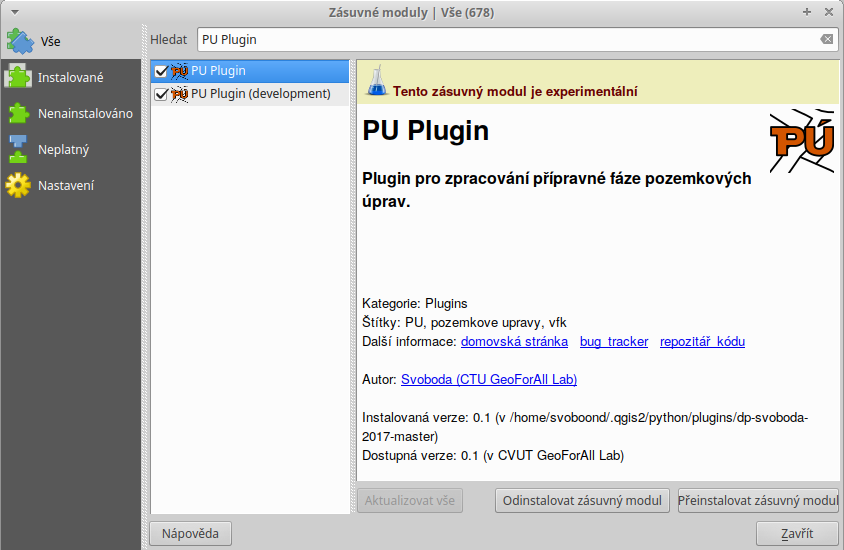
\includegraphics[width=.8\textwidth]{./pictures/instalace_puplugin.png}
		\caption[Instalace zásuvného modulu]{Instalace zásuvného modulu}
		\label{fig:instalace_puplugin}
 	\end{figure}

Když je plugin nainstalován, objeví se v~liště zásuvných modulů jeho ikona (viz obr.~\ref{fig:ikona_puplugin}). Okno zásuvného modulu je možné vyvolat poklepáním na~jeho ikonu nebo volbou \textit{Zásuvné moduly $\rightarrow$ PU Plugin $\rightarrow$ PU Plugin}.

	\begin{figure}[H]
		\centering
		
\includegraphics[width=.1\textwidth]{./pictures/puplugin.png}
		\caption[Plugin - ikona]{Plugin - ikona}
		\label{fig:ikona_puplugin}
 	\end{figure}

\section{Grafické uživatelské rozhraní}
\label{manual_gui}

	\begin{figure}[H]
		\centering
		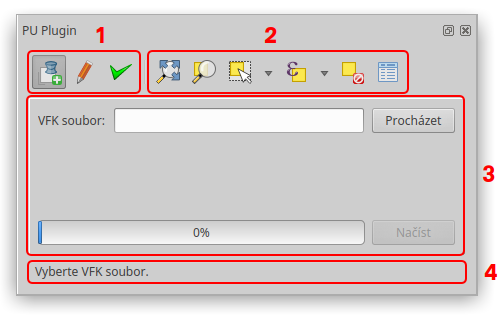
\includegraphics[width=.55\textwidth]{./pictures/main_gui.png}
		\caption[Zásuvný modul - grafické uživatelské rozhraní]{Zásuvný modul - grafické uživatelské rozhraní}
		\label{fig:manual_main_gui}
 	\end{figure}

\begin{description}
	\item[Prvek 1:] Skupina tří ikon pro~přepínání mezi záložkami:
	\begin{itemize}[leftmargin=1.5cm, noitemsep]
		\item \img{./pictures/loadvfk.png} \textit{Načtení VFK souboru}
		\item \img{./pictures/edit.png} \textit{Editace}
		\item \img{./pictures/checkanalysis.png} \textit{Kontroly a analýzy}
 	\end{itemize} 	
	\item[Prvek 2:] Skupina nástrojů, které jsou propojené se~standardními nástroji programu QGIS.
	\item[Prvek 3:] Okna záložek zobrazující se v~závislosti na~tom, která ze~tří ikon záložek (prvkek~1) je aktivní.
	\item[Prvek 4:] Stavový řádek, ve~kterém se ukazují zprávy.
\end{description}

\newpage

\section{Komunikace s uživatelem}
\label{manual_komunikace}

Zásuvný modul komunikuje s~uživatelem třemi způsoby:

\begin{enumerate}[leftmargin=1.5cm, noitemsep]
	\item \underline{Stavový řádek} (viz prvek~4 obr.~\ref{fig:manual_main_gui}) představuje nejčastější způsob zobrazování zpráv zásuvného modulu. Když nevíte jak postupovat, zde s~největší pravděpodobností najdete potřebné informace. Běžné zprávy mají černou barvu písma, důležíté zprávy se~zobrazují červeně (viz obr.~\ref{fig:manual_dulezita_zprava}).
	
	\begin{figure}[H]
		\centering
		
\includegraphics[width=.23\textwidth]{./pictures/statusbar-red_message.png}
		\caption[Důležitá zpráva ve~stavovém řádku]{Důležitá zpráva ve~stavovém řádku}
		\label{fig:manual_dulezita_zprava}
 	\end{figure}	

	\item \underline{Pole zpráv} je standardní způsob komunikace mezi programem QGIS a~uživatelem. Zobrazuje pole v~horní části mapového okna, které může být nastaveno tak, že po~určité době samo zmizí, nebo vyžaduje manuální zavření. Zásuvný modul využívá této komunikace pouze pro~zobrazení významných zpráv, které by neměly být uživatelem opomenuty (viz obr. \ref{fig:manual_zprava_pole_zprav}).

	\begin{figure}[H]
		\centering
		
\includegraphics[width=.7\textwidth]{./pictures/message_bar-message.png}
		\caption[Zpráva upozornění v poli zpráv]{Zpráva upozornění v poli zpráv}
		\label{fig:manual_zprava_pole_zprav}
 	\end{figure}

	\item \underline{Logování} je posledním prostředkem pro~předávání informací, který zásuvný modul používá. Informace v~anglickém jazyce, zejména chybové hlášky, zapisuje do~vlastní záložky s~názvem \textit{PU Plugin} (viz obr. \ref{fig:manual_logovaci_panel}). Panel logovacích zpráv lze zobrazit kliknutím na~ikonu \img{./pictures/log.png} v~pravém dolním rohu QGISu.

	\begin{figure}[H]
		\centering
		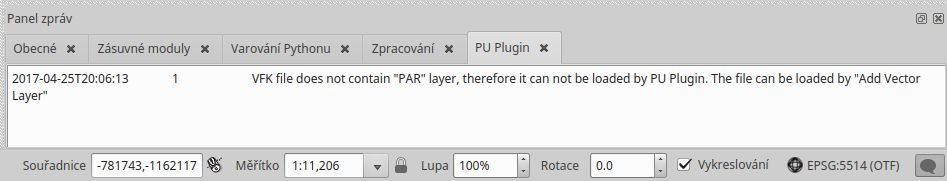
\includegraphics[width=1.0\textwidth]{./pictures/log_panel.png}
		\caption[Panel logovacích zpráv]{Panel logovacích zpráv}
		\label{fig:manual_logovaci_panel}
 	\end{figure}

\end{enumerate}

\newpage

\section{Načtení VFK souboru}
\label{manual_nacteni_vfk}

Záložka \textit{Načtení VFK souboru} slouží k~načtení vrstvy parcel ze~souboru~\zk{VFK} souboru.

	\begin{figure}[H]
		\centering
		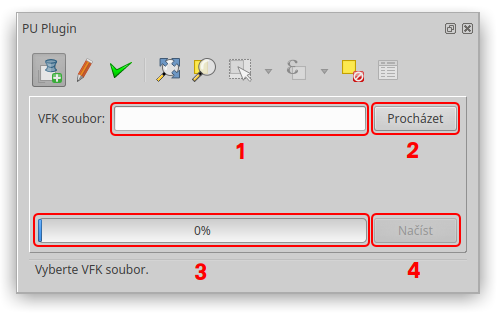
\includegraphics[width=.55\textwidth]{./pictures/nacteni_vfk_gui.png}
		\caption[Záložka \textit{Načtení VFK souboru} - grafické uživatelské rozhraní]{Záložka \textit{Načtení VFK souboru} - grafické uživatelské rozhraní}
		\label{fig:manual_nacteni_vfk_gui}
 	\end{figure}

\begin{description}
	\item[Prvek 1:] Textové pole pro~cestu k~\zk{VFK} souboru.
	\item[Prvek 2:] Tlačítko pro~zobrazení dialogového okna pro~procházení adresářů. Filtruje soubory s~příponou \textit{*.vfk}, pamatuje si poslední použitou cestu.
	\item[Prvek 3:] Indikátor průběhu načítání \zk{VFK} souboru.
	\item[Prvek 4:] Tlačítko pro~načítání \zk{VFK} souboru. Aktivuje se pouze v~případě, že textové pole (prvek~1) obsahuje cestu k~existujícímu \zk{VFK} souboru.
\end{description}

Nejprve je zapotřebí zvolit \zk{VFK} soubor, který chcete načíst. To lze udělat dvěma způsoby. Buď kliknete na~tlačítko \textit{Procházet} (prvek~2), vyberete požadovaný soubor a~cesta k~souboru se automaticky zapíše do~textového pole (prvek~1), nebo zkopírujete cestu k~\zk{VFK} souboru přímo do~zmíněného textové pole. Když se v~textovém poli nachází cesta k~validnímu \zk{VFK} souboru, aktivuje se tlačítko \textit{Načíst} (prvek~4) a~můžete zahájit import. O~průběhu načítání vás informuje indikátor průběhu (prvek~3) a~zprávy ve~stavovém řádku.

Symbologie načtené vrstvy parcel se řídí podle druhu pozemku. Při měřítku 1:4000 a~větším přiblížení se zobrazí parcelní čísla, viz obr. \ref{fig:manual_symbologie_par}.

	\begin{figure}[H]
		\centering
		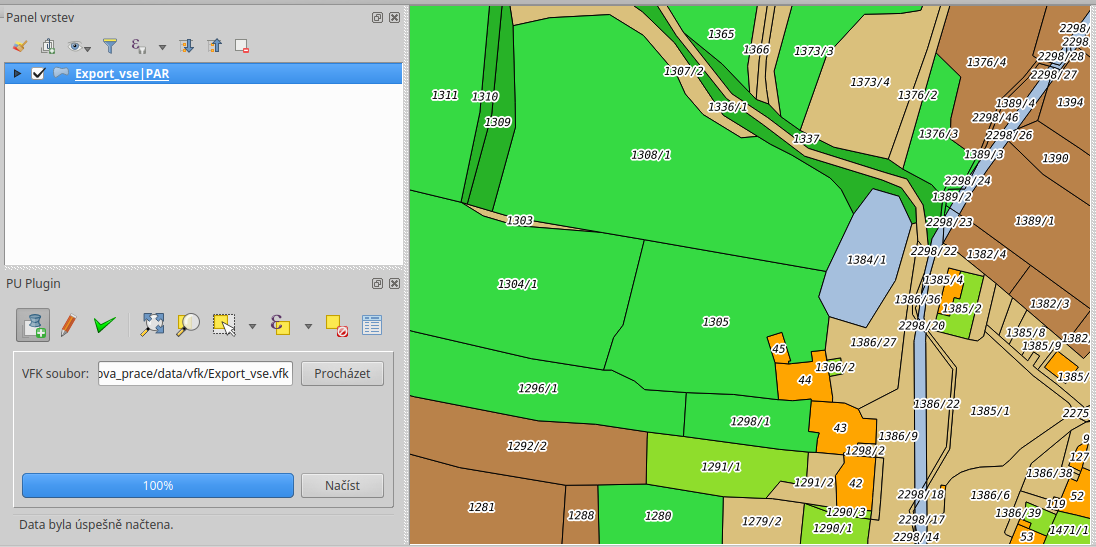
\includegraphics[width=.9\textwidth]{./pictures/symbologie_par.png}
		\caption[Symbologie vrstvy parcel]{Symbologie vrstvy parcel}
		\label{fig:manual_symbologie_par}
 	\end{figure}

Zásuvný modul v~atributové tabulce kvůli přehlednosti skrývá všechny nepotřebné sloupce. Pro~větší srozumitelnost mají viditelné sloupce aliasy.

\newpage

\section{Editace}
\label{manual_editace}

Po úspěšném nahrání vrstvy parcel lze začít s~editací. Záložka \textit{Editace} poskytuje nástroje k~úpravě geometrie a~zařazení parcel do~kategorií.

	\begin{figure}[H]
		\centering
		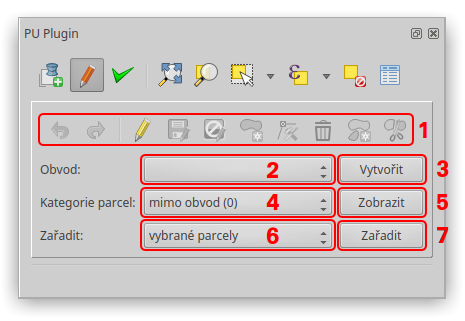
\includegraphics[width=.55\textwidth]{./pictures/editace_gui.png}
		\caption[Záložka \textit{Editace} - grafické uživatelské rozhraní]{Záložka \textit{Editace} - grafické uživatelské rozhraní}
		\label{fig:manual_editace_gui}
 	\end{figure}

\begin{description}
	\item[Prvek 1:] Skupina nástrojů pro~editaci, které jsou propojené se~standardními nástroji programu QGIS.
	\item[Prvek 2:] Rozbalovací menu s~aktuálně načtenými polygonovými vrstvami.
	\item[Prvek 3:] Tlačítko pro~zobrazení dialogového, ve~kterém lze zvolit adresář a~název vrstvy obvodu. Filtruje soubory s~příponou \textit{*.pu.shp}, pamatuje si poslední použitou cestu.
	\item[Prvek 4:] Rozbalovací menu s~kategoriemi parcel. Na~výběr jsou tyto kategorie, číslo v~závorce udává hodnotu, kterou zásuvný modul pro~kategorii používá:
	\begin{itemize}[leftmargin=1.5cm, noitemsep]
		\item \textit{mimo obvod (0)}
		\item \textit{v~obvodu - neřešené (1)}
		\item \textit{v~obvodu - řešené (2)}
		\item \textit{bez kategorie}
	\end{itemize}
	\item[Prvek 5:] Tlačítko pro~zobrazení (výběr) parcel v~aktuálně zvolené kategorii.
	\item[Prvek 6:] Rozbalovací menu s~variantami zařazení parcel. K~dispozici jsou dvě možnosti:
	\begin{itemize}[leftmargin=1.5cm, noitemsep]
		\item \textit{vybrané parcely} - zařadí vybrané parcely do~aktuálně zvolené kategorie.
		\item \textit{obvodem} - zařadí všechny parcely do~kategorií na~základě obvodu.
	\end{itemize}
	\item[Prvek 7:] Tlačítko pro~provedení zařazení.
\end{description}

Zásuvný modul pracuje s~aktivní vrstvou, tj. vrstva vybraná v~panelu vrstev, který se ve~výchozím nastavení nachází na~levé straně okna.

Vrstvu parcel je možné editovat pomocí sady standardních nástrojů v~horní části pluginu (prvek~1).

Nejdůležitější funkcionalitou této záložky je ovšem zařazení parcel do~kategorií. Aby bylo na~první pohled zřejmé, ve~které kategorii jsou jednotlivé parcely zařazeny, používá zásuvný modul tzv.~vrstvu obvodu. Jedná se o~samostatnou vrstvu ve~formátu \textit{shapefile}. Pro~odlišení od~jiných dat mají vrstvy obvodu příponu \textit{*.pu.shp}. Adresář a~název této vrstvy můžete specifikovat pomocí tlačítka \textit{Vytvořit} (prvek~3). Po~poklepání na~zmíněné tlačítko se otevře dialogové okno, kde lze zvolit umístění vrstvy obvodu. Z~aktivní vrstvy, která musí být \zk{VFK}, se vytvoří vrstva obvodu, zásuvný modul ji načte a~vybere v~rozbalovacím menu (prvek~2).

Pokud cesta k~vrstvě obvodu není uživatelem definována (rozbalovací menu je prázdné), nebo je v~rozbalovací menu vybrána vrstva, která nebyla vytvořena zásuvným modulem a~tudíž neobsahuje potřebné sloupce, plugin automaticky vytvoří vrstvu obvodu ve~stejném adresáři, ve~kterém se nachází aktivní vrstva parcel.

Funkce pro~vytvoření obvodu je volána v~momentě, kdy je pro~vrstvu parcel uložena změna geometrie, uložena změna, při~které došlo k~vymazání prvku, nebo je pomocí tlačítka \textit{Zařadit} (prvek~7) provedeno zařazení parcel.

Pro symbologii vrstvy obvodu byla zvolena červená barva, popisky obsahují pouze číslo kategorie, viz obr.~\ref{fig:manual_symbologie_obvod}.

	\begin{figure}[H]
		\centering
		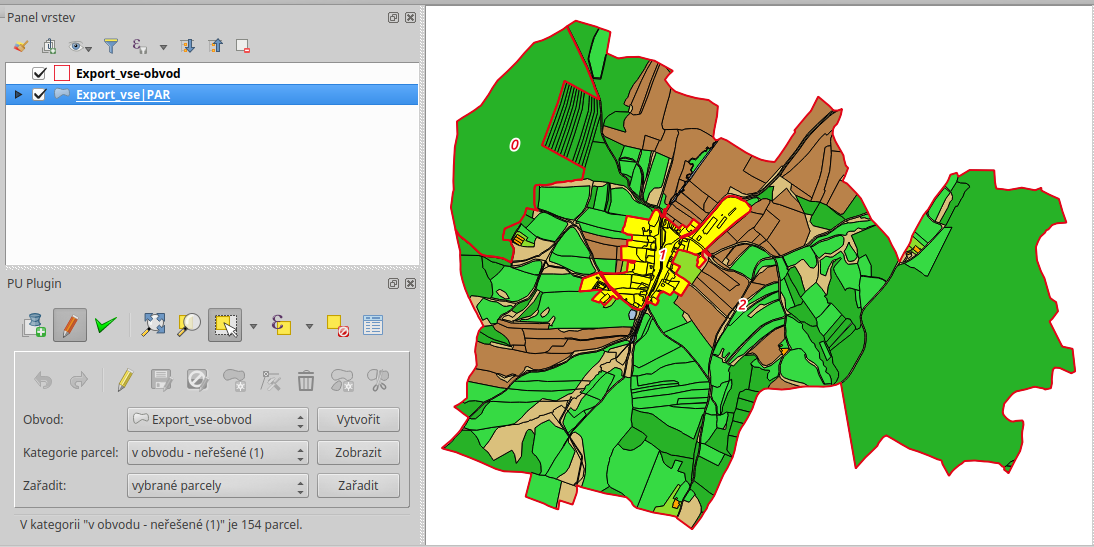
\includegraphics[width=1.0\textwidth]{./pictures/symbologie_obvod.png}
		\caption[Symbologie vrstvy obvodu]{Symbologie vrstvy obvodu}
		\label{fig:manual_symbologie_obvod}
 	\end{figure}

Zásuvný modul nabízí dvě varianty zařazení parcel (prvek~6). První možností je volba \textit{vybrané parcely}, která provede zařazení vybraných parcel do~zvolené kategorie (prvek~4).

Druhý způsob nazvaný \textit{obvodem} rozřadí všechny parcely ve~\zk{VFK} vrstvě do~kategorií. Jako podklad použije aktuálně vybranou vrstvu obvodu (viz prvek~2). Tato varianta pracuje pouze s~obvody, které vytvořil zásuvný modul pro~pozemkové úpravy. Pro~zařazení do~kategorie musí být parcela kompletně uvnitř geometrie příslušného prvku obvodu.

Pro kontrolu nabízí zásuvný modul tlačítko \textit{Zobrazit} (prvek~5), které vybere, a~tím pádem zvýrazní, prvky v~kategorii.

Pokud vytvoříte novou parcelu, nebo~pomocí nástroje \textit{Přidat část} doplníte popisné údaje o~geometrii, vyplňte měřítko podkladů do~sloupce \textit{MERITKO PODKL.}. Tento údaj používá kontrola \textit{výměra nad mezní odchylkou}.

\newpage

\section{Kontroly a analýzy}
\label{manual_kontroly_analyzy}

Poslední záložka zásuvného modulu nabízí možnost zkontrolovat data, zejména soulad mezi~\zk{SPI} a~\zk{SGI}, a~provést analýzy nezbytné pro~sestavení nárokových listů.

	\begin{figure}[H]
		\centering
		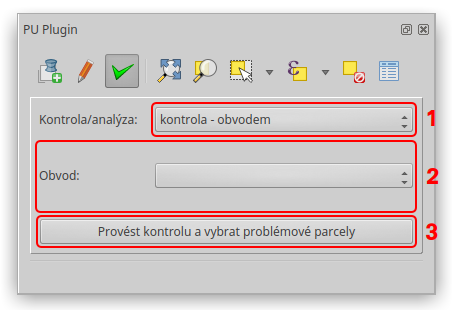
\includegraphics[width=.55\textwidth]{./pictures/ca_gui.png}
		\caption[Záložka \textit{Kontroly a analýzy} - grafické uživatelské rozhraní]{Záložka \textit{Kontroly a analýzy} - grafické uživatelské rozhraní}
		\label{fig:manual_ca_gui}
 	\end{figure}

\begin{description}
	\item[Prvek 1:] Rozbalovací menu pro~přepínání mezi kontrolami a~analýzami.
	\item[Prvek 2:] Okna kontrol a~analýz zobrazující se v~závislosti na~tom, která položka rozbalovacího menu (prvek~1) je vybrána.
	\item[Prvek 3:] Tlačítko pro~provedení kontroly či~analýzy.
\end{description}

V~rozbalovacím menu (prvek~1) zvolte kontrolu či~analýzu, důsledkem čehož se změní dolní okno (prvek~2). Když je vše potřebné zadané, lze kontrolu či~analýzu spustit. Zprávy ve~stavovém řádku poskytují informace o~výledku.

\subsubsection{Kontrola - obvodem}
\label{manual_kontrola_obvodem}

Kontrola obvodem provádí výběr parcel, které nejsou kompletně uvnitř vrstvy obvodu.

Jestliže od~začátku pracujete pouze s~jednou vrstvou obvodu, měl by být výsledek této kontroly stejný jako při~zvolení kategorie \textit{bez kategorie} (viz prvek~4 na~obr.~\ref{fig:manual_editace_gui}) a~provedení výběru prvků v~kategorii pomocí tlačítka \textit{Zobrazit} (viz prvek~5 na~obr.~\ref{fig:manual_editace_gui}). Lišit se tyto dvě metody budou v~momentě, kdy si do~QGISu nahrajete vrstvu obvodu, kterou jste vytvořili s~jinou vrstvou parcel. Jinými slovy tato kontrola používá geometrii vrstvy obvodu a~tlačítko \textit{Zobrazit} v~záložce \textit{Editace} vybírá parcely na~základě údajů uložených v~atributové tabulce.

Jediným potřebným vstupem je zmiňovaná vrstva obvodu v~rozbalovacím menu (viz obr.~\ref{fig:manual_kontrola_obvodem_gui}), které je propojené s~menu vrstvy obvodu v~záložce \textit{Editace}.

	\begin{figure}[H]
		\centering
		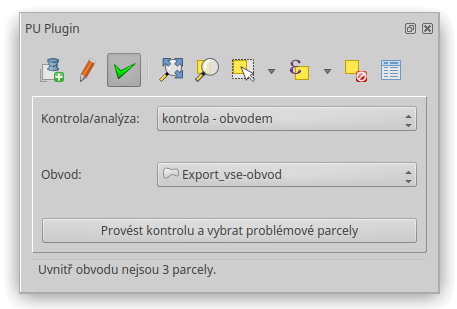
\includegraphics[width=.55\textwidth]{./pictures/kontrola-obvodem.png}
		\caption[Kontrola \textit{obvodem} - grafické uživatelské rozhraní]{Kontrola \textit{obvodem} - grafické uživatelské rozhraní}
		\label{fig:manual_kontrola_obvodem_gui}
 	\end{figure}

\subsubsection{Kontrola - není v SPI}
\label{manual_kontrola_neni_v_spi}

Kontrola \textit{není v SPI} slouží k~zobrazení parcel, které nejsou v~souboru popisných informací.

\subsubsection{Kontrola - není v mapě}
\label{manual_kontrola_neni_v_mape}

Kontrola \textit{není v~mapě} vybírá parcely, které mají nulovou geometrii a~tudíž se nezobrazují v~mapovém okně.

\subsubsection{Kontrola - výměra nad mezní odchylkou}
\label{manual_kontrola_vymera}

Kontrola \textit{výměra nad~mezní odchylkou} ověřuje, zda~rozdíl mezi výměrou dle~\zk{SPI} a~výměrou vypočtenou z~\zk{SGI} nepřekračuje mezní odchylku. Ta je stanovena katastrální vyhláškou a~závisí na~kódu kvality nejméně přesně určeného lomového bodu na~hranici parcely. Jestliže je parcela digitalizovaná, kód kvality podrobných bodů se určí podle~měřítka podkladové mapy, viz sloupec \textit{MERITKO PODKL.}.

\subsubsection{Kontrola - bez vlastníka}
\label{manual_kontrola_bez_vlastnika}

Kontrola \textit{bez~vlastníka} vybírá parcely, které jsou bez~vlastníka, tzn. že~nemají přiřazený list vlastnictví.

\subsubsection{Analýza - měření vzdálenosti}
\label{manual_analyza_vzdalenosti}

Analýza \textit{měření vzdálenosti} počítá pro~všechny řešené parcely vzdálenost jejich těžiště od~referenčního bodu. Výsledné zaokrouhlené hodnoty v~metrech ukládá do sloupce \texttt{VZDALENOST}.

Pro~spuštění této kontroly je zapotřebí v~rozbalovacím menu, které filtruje bodové vrstvy, zvolit vrstu referenčního bodu, viz obr.~\ref{fig:manual_analyza_vzdalenosti_gui}. Vybraná vrstva referenčního bodu musí obsahovat právě jeden prvek a~musí mít stejný souřadnicový systém jako vrstva parcel.

	\begin{figure}[H]
		\centering
		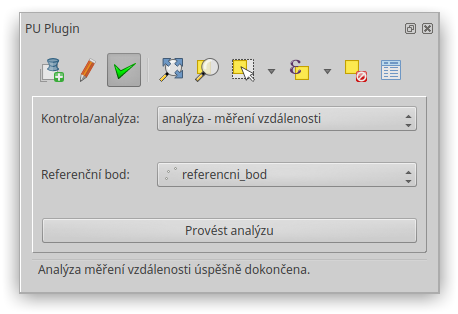
\includegraphics[width=0.55\textwidth]{./pictures/analyza_vzdalenost.png}
		\caption[Analýza \textit{měření vzdálenosti} - grafické uživatelské rozhraní]{Analýza \textit{měření vzdálenosti} - grafické uživatelské rozhraní}
		\label{fig:manual_analyza_vzdalenosti_gui}
 	\end{figure}

\subsubsection{Analýza - oceňování podle BPEJ}
\label{manual_analyza_bpej}

Analýza \textit{oceňování podle BPEJ} počítá cenu pozemku na~základě vrstvy hranic \zk{BPEJ}.

	\begin{figure}[H]
		\centering
		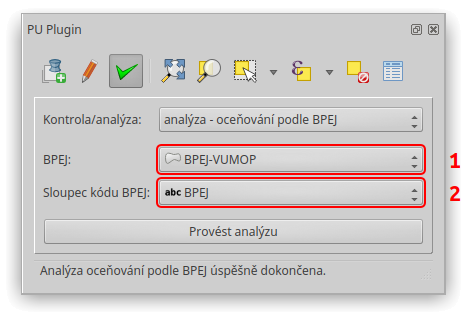
\includegraphics[width=0.55\textwidth]{./pictures/analyza_bpej.png}
		\caption[Analýza \textit{oceňování podle BPEJ} - grafické uživatelské rozhraní]{Analýza \textit{oceňování podle BPEJ} - grafické uživatelské rozhraní}
		\label{fig:manual_analyza_bpej_gui}
 	\end{figure}

\begin{description}
	\item[Prvek 1:] Rozbalovací menu s~aktuálně načtenými polygonovými vrstvami.
	\item[Prvek 2:] Rozbalovací menu se~sloupci vybrané vrstvy \zk{BPEJ}.
\end{description}

Vyberte vrstvu hranic \zk{BPEJ} (prvek~1) a~poté zvolte sloupec, ve~kterém jsou uloženy kódy \zk{BPEJ}. Vrstva hranic \zk{BPEJ} musí mít stejný souřadnicový systém jako vrstva parcel.

Pro určení ceny za~metr čtvereční jednotlivých kódů \zk{BPEJ} analýza používá číselník \zk{BPEJ} z~Českého úřadu zeměměřičského a~katastrálního.

Do~atributové tabulky se zápíše nejen cena celková (sloupec CELK. CENA), ale~také cena za~metr čtvereční, výměra a~cena dle jednotlivých bonit v~příslušné parcele (sloupec  BPEJ KOD-CENA ZA M2-VYMERA-CENA). Pokud omylem zvolíte špatný sloupec, nebo když kód \zk{BPEJ} není nalezen v~číselníku, zásuvný modul vybere ve~vrstvě obvodu prvky, pro~které nenalezl ceny, a~informuje vás o~problému.
